% !TEX root =  master.tex
\cleardoublepage
\chapter{PCR-Pooling}
\section{Parameter und Kenngrößen für das Verfahren}
%Prävalenz
\begin{wrapfigure}{r}{0.44\textwidth}
	%\centering
	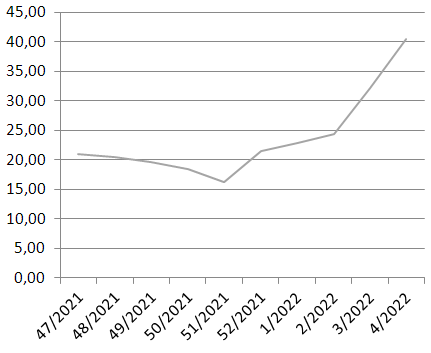
\includegraphics[width=.44\textwidth]{img/RKI_PCR_Positivrate}
	\caption{Prävalenz von PCR-Tests}
\end{wrapfigure}
Die \textbf{Prävalenz} ist die Quote, mit welcher eine Krankheit in einer Stichprobe vorkommt.\footnote{Leon Gordis S37}
Sie ist ähnlich der derzeit allgemein bekannteren Inzidenz, welche sich auf die Gesamtbevölkerung bezieht.
Bei einer anlasslosen, repräsentativen Testung der Bevölkerung kann die Prävalenz eines Tests gleich der Inzidenz sein.
Bei einer anlassbezogenen Testung werden allerdings meist deutlich höhere Prävalenzen beobachtet.
Gemäß aktuellem RKI-Wochenbereicht sind zwischenzeitlich über 40 Prozent der PCR-Tests positiv.
\footnote{RKI Wochenbericht}

%Mögliche Poolgrößen
Das PCR-Verfahren erlaubt grundsätzlich ein \textbf{Pooling} von mehreren Testpersonen.
Die Proben der Patienten werden hierbei zu einem Pool zusammengefasst und gemeinsam getestet.
Das PCR-Verfahren ist darauf ausgelegt, geringe DNA-Mengen zu einer nachweisbaren Menge zu vermehren.
Die Verwässerung der Probe ist bis zu einem gewissen Punkt deshalb unproblematisch für den Nachweis.
Auch eine (zu) hohe Verdünnung ist zulasten der Erkennungsrate problemlos möglich.
Abgewogen werden muss hierbei die Priorisierung zwischen Präzision und Kostenersparnis.
Eine Poolgröße von bis zu 20 Personen liegt laut Viehweger "comfortable above the detection rate"\footnote{Vieweger v1}
Andere Gruppe halten Poolgrößen von bis zu 90 Personen für akzeptabel.\footnote{Quelle 2 Pooling Verwässerung}
Es ist zu beachten, dass bei größeren Pools mehr Verdopplungsschritte notwendig sind, um dieselbe Virenmenge in der Probe zu erhalten.
Beim Pooling von 16 Personen liegt beispielsweise eine um $2^{4}$ niedrigere Virenlast vor.
Deshalb müssen 4 weitere Zyklen eingeplant werden.
\footnote{Vieweger v1}

\section{Umgang mit dem Ergebnis}
\begin{wrapfigure}{r}{0.4\textwidth}
	%\centering
	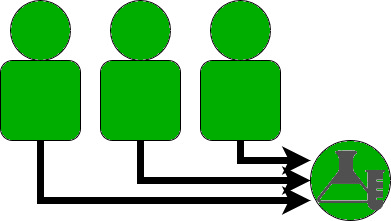
\includegraphics[width=.4\textwidth]{img/PoolAlleNegativ}
	\caption{Pooling benötigt für drei negative Personen nur ein Test}
\end{wrapfigure}
\textbf{Ergebnisinterpretation}
\begin{itemize}
	\item \textbf{Negatives Poolergebnis:}\newline
	Ein negatives Gesamtergebnis bedeutet, dass \textbf{jede Einzelprobe negativ} war.
	Es wurde somit durch einen Test festgestellt, dass alle Personen im Pool negativ sind.
		
	\item \textbf{Positives Poolergebnis:}\newline
	Ein positives Gesamtergebnis bedeutet, dass \textbf{mindestens eine Einzelprobe positiv} war.
	In diesem Fall müssen weitere Tests durchgeführt werden, um die positiven Einzelpersonen zu ermitteln.

\end{itemize}

\begin{wrapfigure}{r}{0.4\textwidth}
	%\centering
	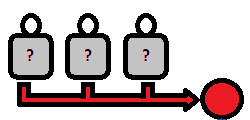
\includegraphics[width=.4\textwidth]{img/PoolPositiv}
	\caption{Ein positiven Pool kann die positive Person nicht idendifizieren}
\end{wrapfigure}
\textbf{Unklare Ergebnisse}\newline
Durch Pooling besteht das Risiko, dass die Ergebnisse nicht für alle Testpersonen eindeutig interpretiert werden können.
Wie häufig dies der Fall ist und welcher Anteil der Testgruppe nachuntersucht werden muss, ist abhängig vom gewählten Verfahren.

Hierdurch werden \textbf{Nachtestungen} der betroffenen Personen notwendig.
Die Tests erfolgen hierbei nacheinander und sind statistisch unabhängig voneinander.
Manche Verfahren erfordern sogar mehrere sequenzielle Nachtestungen.

Um Nachtestungen zu ermöglichen, müssen die Proben ausreichend Substanz für mehrere Testungen enthalten.
Durch die erneute Testung verlängert sich der Zeitraum, bevor für alle Testpersonen das Ergebnis fest steht.
Dies kann abhängig von der Situation in welcher der Test benötigt wird nicht akzeptabel sein.

\cleardoublepage
\begin{wrapfigure}{r}{0.4\textwidth}
	%\centering
	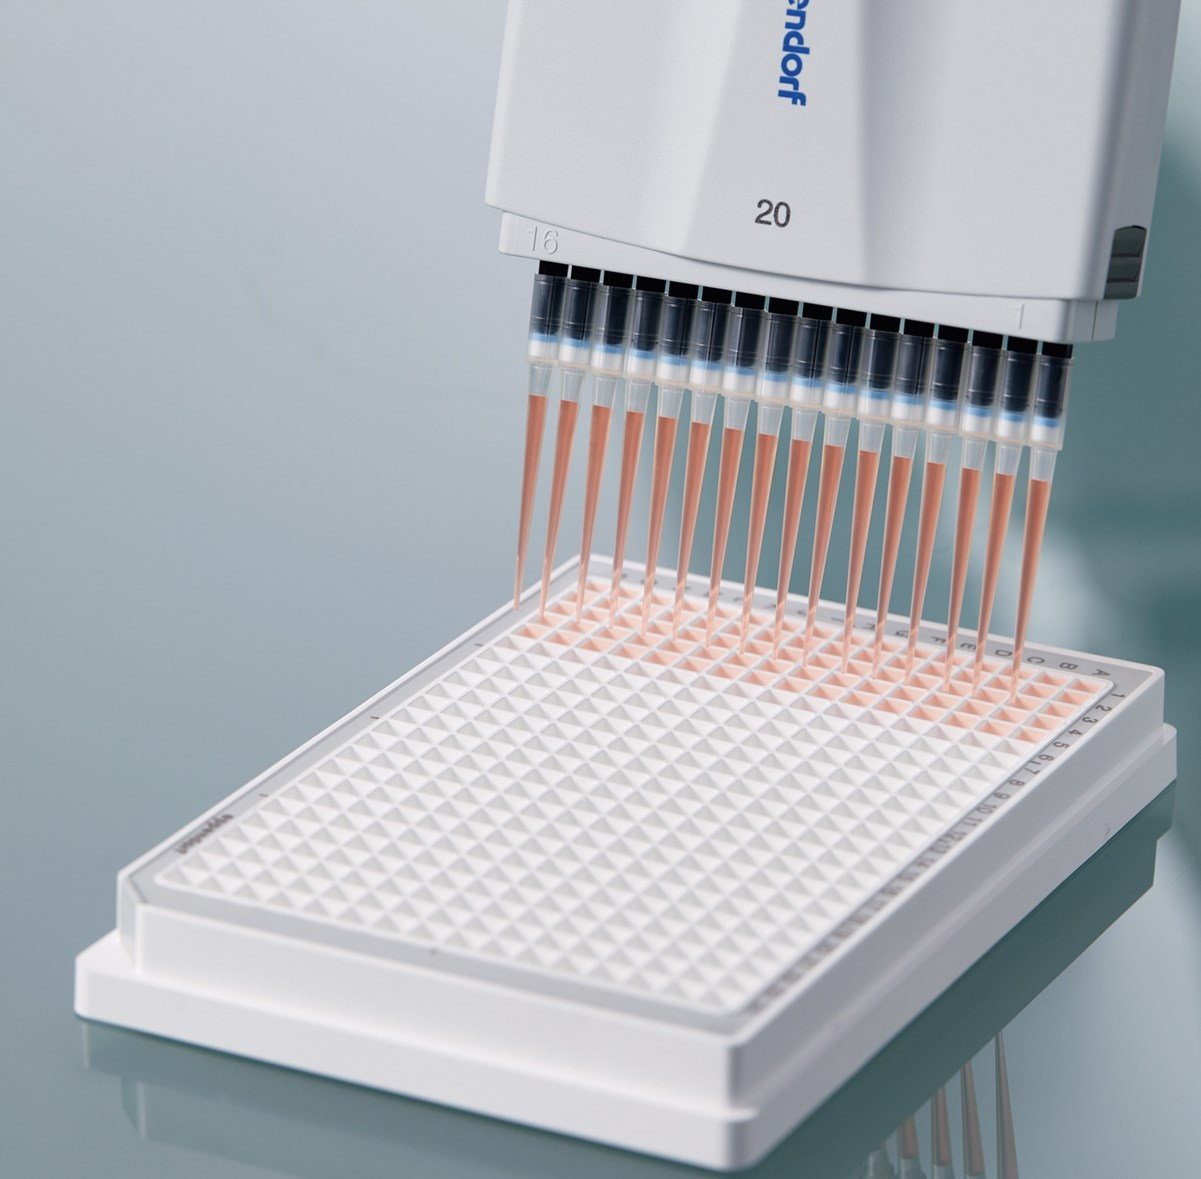
\includegraphics[width=.4\textwidth]{img/Pipettenmatrix}
	\caption{Pipettenautomat}
\end{wrapfigure}
Beim ersten Poolingdurchlauf muss darauf geachtet werden, die Proben untereinander nicht zu kontaminieren.
Eine Verunreinigung der Originalproben würde eine spätere Nachtestung unmöglich machen.

Um eine \textbf{Kontamination} durch das Pooling zu verhindern, sollte die komplette Matrix vor dem Pooling einmal dupliziert werden. 
Die für den aktuellen Test notwendigen Proben werden hierbei entnommen und im Duplikat gepoolt.
Für diesen Duplikationsschritt gibt es spezialisierte Laborgeräte, sodass dies in einem Arbeitsschritt für alle Proben durchgeführt werden kann - teilweise sogar automatisiert.\footnote{https://www.genengnews.com/wp-content/uploads/2019/07/Eppendorf.jpg}

\begin{wrapfigure}{l}{0.4\textwidth}
	%\centering
	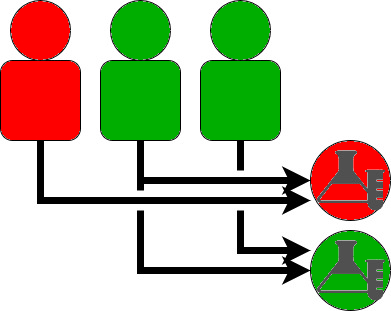
\includegraphics[width=.4\textwidth]{img/KomplexePools}
	\caption{Überlappende Pools}
	
	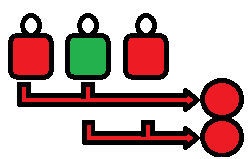
\includegraphics[width=.4\textwidth]{img/MehrerePositiv}
	\caption{Mehrere Positivfälle}
\end{wrapfigure}

\textbf{Überlappende Pools}\newline
Um das Problem der Nachtestungen zu lösen, kann man mehrere überlappende Tests durchführen.
Aus der Kombination der Ergebnisse ist es theoretisch möglich, die infizierte Person zu triangulieren.

Schwierig wird es hierbei, wenn mehrere Personen innerhalb der Testgruppe positiv sind.
Die positiven Tests lassen sich dann nicht mehr exakt einer Person zuordnen.

Das Ergebnis in Abbildung X.X legt nahe, dass die mittlere Person infiziert ist.
Beide Pools fallen positiv aus und nur die mittlere Person ist Teil beider Testgruppen.
Für diese Person wäre es somit naheliegend ein falsch-positives Ergebnis mitzuteilen.

Die Kosten der Testung haben sich zudem für alle Testgruppen erhöht, da durch diese Strategie für die erste Testrunde bereits zwei Tests notwendig sind, um eine Testgruppe von drei Personen abzubilden.

\cleardoublepage
\begin{figure}[h]
	\centering
	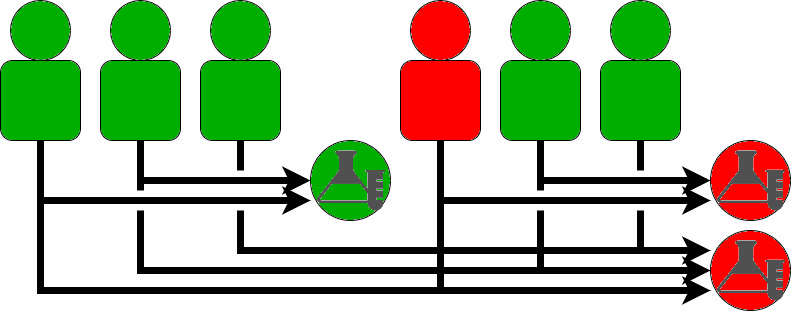
\includegraphics[width=.8\textwidth]{img/GrossePooluebersicht}
	\caption{Überlappende Pools}
\end{figure}

Weitere Schwierigkeiten ergeben sich, wenn für Personen gemischte Ergebnisse vorliegen.
Bei den drei Personen der rechten Testgruppe sind als beide Pooltests positiv ausgefallen.
In dieser Gruppe sind höchstwahrscheinlich eine oder mehrere Personen infiziert und die Gruppe muss nachgetestet werden.

Bei den Personen der linken Gruppe liegt allerdings ein positives und ein negatives Ergebnis vor.
Theoretisch kann durch das negative Ergebnis ausgeschlossen werden, dass eine Person dieser Gruppe infiziert ist.
In der Praxis ist allerdings kein Test 100 Prozent zuverlässig.
Für diese Personen liegt somit ein positiver Pool vor und das Negativergebnis könnte fehlerhaft sein.
Testet man nun zur Sicherheit nochmal alle?

Die \textbf{sicherste Variante} wäre, alle Personen nachzutesten die Teil eines positiven Pools waren.
Hierdurch wäre der Mehrwert durch das Pooling allerdings schnell verloren.
Abhängig vom Anwendungsfall kann es dagegen akzeptabel sein, einige Infektionen nicht zu erkennen.
Dies ist bei anlasslosen Massentestungen der Fall sein in denen kein Negativzertifikat ausgestellt wird.
Die Kostenoptimierung steht hierbei im Vordergrund, sodass \textbf{einige falsch-negative Ergebnisse akzeptabel} sein können. 

In der Praxis sollte meist ein Mittelweg gewählt werden.
Dieser könnte beispielsweise sein, alle mutmaßlich negativen Personen einer Testgruppe in einem gemeinsamen Pool nachzutesten.
Dieser Pool hat damit eine erwartete Prävalenz von null und sollte immer negativ ausfallen.
Hierdurch kann ermittelt werden, ob beim ersten Durchlauf Fehler passiert sind und Personen übersehen wurden.
Sollte dieser Pool positiv werden, müssen alle Teilnehmer einzeln nachgetestet werden.
Hierduch werden bereits drei sequenzielle Durchläufe notwendig
Die Übermittlung des Testergebnisses wird hierdurch stark verzögert, was ebenfalls Probleme verursachen kann.

\section{Ermittlung des Erwartungswertes}
\begin{wrapfigure}{r}{0.4\textwidth}
	%\centering
	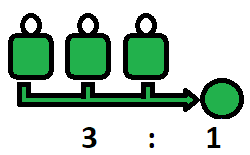
\includegraphics[width=.4\textwidth]{img/EffizienzNegativ}
	\caption{Effizienz eines \newline negativen Pools}
	
	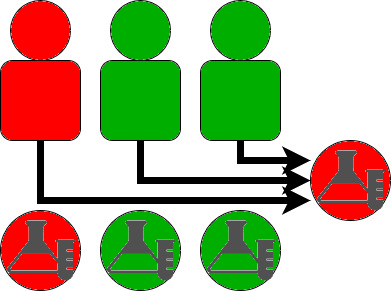
\includegraphics[width=.4\textwidth]{img/EffizienzPositiv}
	\caption{Effizienz eines \newline positiven Pools}
\end{wrapfigure}

Als \textbf{Effizienz} einer Poolingmethode wird nachfolgend der Multiplikator bezeichnet, welcher gegenüber Einzeltestungen erzielt werden kann.
Diese ist Abhängig von der Größe der Testgruppe und der Anzahl der Tests die erforderlich sind um den Infektionsstatus jeder Person zu klassifizieren.
Die Effizienz lässt sich somit beschreiben als $\frac{Anzahl Testpersonen}{Anzahl Tests} $.

Im bestmöglichen Fall ist die gesamte Testgruppe nicht infiziert.
Hierdurch fallen im ersten Durchlauf alle Tests negativ aus und die gesamte Testgruppe kann als negativ markiert werden.
Im Beispiel der Abbildung X.X ergibt sich eine Effizienz von 3.

Im Falle einer Nachtestung wird ein initialer Test für den Pool benötigt, welcher positiv ausfällt.
Danach werden nochmal Tests für jede Einzelperson benötigt.
Die Effizienz lässt sich somit beschreiben als $\frac{Anzahl Testpersonen (N)}{1 Pooltest + N Einzeltests} $.
Für den Positivfall liegt die Effizienz also bei 0,75.
Das Ergebnis ist damit schlechter als wenn direkt einzeln getestet worden wäre, da zuerst ein zusätzlicher Pooltest verwendet wurde.

Für den Vergleich von Teststrategien ist der \textbf{Erwartungswert für die Effizienz} relevant.
Die benötigte Anzahl der Tests ist abhängig vom Ergebnis der Pooltests.
Wenn alle Ergebnisse negativ sind, ist die Effizienz 3. Wenn das Poolergebnis positiv ist, liegt die Effizienz bei nur 0,75.
Der Erwartungswert ergibt sich aus diesen beiden Szenarien, gewichtet nach ihrer Eintrittswahrscheinlichkeit.
Die Wahrscheinlichkeit, dass jemand innerhalb der Testgruppe Infiziert ist, hängt von der Prävalenz und der Größe der Testgruppe ab.

Bei einer Prävalenz von 10 Prozent und drei statistisch unabhängigen Testpersonen, liegt die Wahrscheinlichkeit für einen Positivfall bei 30 Prozent. \textbf{Statistik prüfen}
Die Effizienz liegt also mit einer Wahrscheinlichkeit von 30 Prozent bei 0,75 und mit einer Wahrscheinlichkeit von 70 Prozent bei 3,0.
Daraus ergibt sich unter diesen Parametern eine gewichtete Effizienz für das Verfahren von 2,325.

\cleardoublepage
